\input{../common}

\begin{document}
  %<*content>
  \lesson{analysis}{29}{Statistique à deux variables}
  
 
 L'étude conjointe de deux variables statistiques sur une même population est fréquente dans le domaine des sciences exactes comme dans celui des sciences humaines. \\On cherche alors à déterminer s'il existe un lien entre ces deux variables et, le cas échéant, quelle est la nature de ce lien.
La première étape consiste à représenter sur un même graphique les deux variables statistiques. C'est ce que l'on appelle tracer un nuage de points. On regarde ensuite si ce nuage de points se rapproche d'une courbe connue, afin de déterminer la nature du lien (ou la \textbf{corrélation}) éventuel entre les deux variables statistiques.\\
La notion de corrélation semble avoir été esquissée pour la première fois par  le britannique  Francis Galton, (1822-1911), dans ses travaux sur l'hérédité.\\
En 1886, il examinait la taille des enfants en fonction de la taille moyenne des parents. Il nota que les enfants de parents de grande taille
avaient tendance à être plus petits qu'eux. Il y avait donc régression du
caractère "grande taille" :  la droite d'ajustement de y en x qu'il utilisa fut nommée droite de régression. C'est pourquoi   la droite d'ajustement affine est  appelée  droite de régression linéaire.\\

\subsection{Statistique à une variable - Rappels}
\subsection*{Moyenne - Variance - Écart-type}
Soit X un caractère étudié dans une population d'effectif n,\; prenant les valeurs $ x_{1} $ ,  $ x_{2} $,   $ x_{3}$, $ \cdots $, $x_{n}$.\\
%A chaque modalité $ x_{i} $ on associe son effectif $ n_{i} $.\\
%$n_{1} + n_{2} + \cdots+ n_{p}  =  N$\; ( effectif total)


\begin{definition}

\begin{itemize}
\item[$  \bullet$] L'ensemble des réels $x_i$ est appelé série statistique simple ou série statistique à une variable.
%\item[$  \bullet$] \textbf{La fréquence} de la modalité $x_i$ est le réel noté $f_i$ tel que : $f_i = \frac{n_i}{N}$
\item[$  \bullet$] La    \textbf{moyenne} de la série statistique est le réel noté  $ \overline{x} $ ou       $ \overline{X} $ tel que : $$ \overline{x} = \frac{x_{1}+x_{2}+\cdots +x_{n}}{n}$$
\item[$  \bullet$] La  \textbf{variance} de la série statistique  est le réel noté  $V(x)$ ou $V(X)$ tel que :
$$ V(x) = \frac{x_{1}^{2}+x_{2}^{2}+\cdots +x_{n}^{2}}{n}-\overline{x}^{2}$$
\end{itemize}
L'\textbf{écart-type} est la racine carrée de la variance. On le note  $ \sigma _{x} $ ou $ \sigma_X $. $$ \sigma_x=\sqrt{V(x)} $$
\end{definition}





\medskip

\begin{example}

On considère la série de notes d'élèves de TS1, à un devoir de maths.
\begin{center}
   $\begin{array}{|c|c|c|c|c|c|c|c|c|}
\hline
 Notes  x_{i}  & 7&  14&13&15&  10 &8 &9& 11 \\
\hline
\end{array}$
\end{center}




\medskip

 On a: \; $$  \overline{x}=\dfrac{7+ 14+13+15+  10 +8 +9+ 11}{8} =\dfrac{87}{8}=10,875$$ 
 
 La variance est alors :
 
 $$  V(x)=\dfrac{7^{2}+ 14^{2}+13^{2}+15^{2}+  10^{2} +8^{2} +9^{2}+ 11^{2}}{8}-10,875^{2} $$ 
  $$  V(x)=\dfrac{49+ 196+169+225+  100 +64 +81+ 121}{8}-118,26563 $$ 
    $$  V(x)=\dfrac{1005}{8}-118,26563 $$ 
    $$  V(x)=  125,625-118,26563$$ 
    $$  V(x)=7,35937$$ 
    
   D'où l'écart-type:
    $$ \sigma_x=\sqrt{7,35937}\approx2.713$$
\end{example}


\subsection{Série statistique à deux variables}
On considère dans une même  population d'effectif $ n $, deux caractères  quantitatifs $X$ et $Y$ prenant respectivement les valeurs  $x_1,\; x_2,\cdots,\;x_n$\; et \;  $  y_1,\; y_2, \cdots,\; y_n$. \\  A chaque individu de la population , on associe un  couple $(x_i,y_i)$.\\
L'ensemble des couples $(x_i,y_i)$ est appelé série statistique double ou à deux variables associée au couple de caractère $(X,Y)$.


\begin{example}

Le tableau ci-dessous donne les notes X de maths et Y de français obtenues par 10 candidats au Bac L.

\begin{center}

  $ \begin{array}{|c|c|c|c|c|c|c|c|c|c|c|}
\hline
  x_i & 7& 8 & 12&  11 &  14  &10 & 15 & 10  &12 & 10\\
 \hline
  y_i  & 8 & 11 & 9 & 13& 13 &9 &17 &12 &11&9 \\
 \hline
\end{array}$
\end{center}

L'effectif du couple $(11 ;13)$ est $1$ . La fréquence du couple $(11 ;13)$ est $\frac{1}{10} =0,1$.\\
L'effectif du couple $(10;9)$ est $2$. La fréquence du couple $(10 ;9)$ est $\frac{2}{10} =0,2$.\\
Les modalités du caractère X sont :
 7-8-10-11-12-14-15.\\
Les modalités du caractère Y sont :
8-9-11-12-13-17.

\end{example}


\subsection*{Nuage de points et point moyen}
Soit $(X,Y)$ une série  statistique double.\\  Dans un plan muni d'un repère
orthogonal, on représente les points de
coordonnées $(x_i ,y_i )$. \\
L'ensemble de ces points est appelé \textbf{nuage} de
la série double.

\begin{example}
\textit{Nuage de la série double de l'exemple précèdent.}

\begin{center}

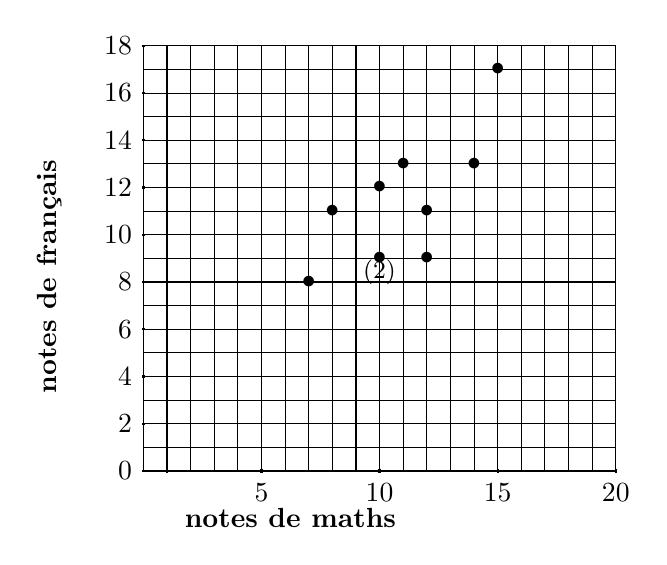
\begin{tikzpicture}[scale= 0.3 ]
\draw  (0,0) grid  (20,18) ;
\foreach\x in {,,,,,5,,,,,10,,,,,15,,,,,,20}
{
\draw[thick] (\x,0.1) -- (\x,-0.1) node[below] {\x};
}
\foreach\y in {0,2,4,6,8,10,12,14,16,18}
{
\draw[thick] (0.05,\y) -- (-0.05,\y) node[left] {\y};
}
\node  at (-4,8)
             {\rotatebox{90}{\bf{ notes de français}}};
  \node  at (6,-2)
             {\rotatebox{0}{\bf{ notes de maths}}};
   \node at(7,8) {$ \bullet $};
   \node at(8,11) {$ \bullet $};
   \node at(10,9) {$ \bullet $ };
   \node at(10,8.4) {\small(2)};
   \node at(10,12) {$ \bullet $};
   \node at(11,13) {$ \bullet $};
    \node at(12,9) {$ \bullet $};
     \node at(12,11) {$ \bullet $};
      \node at(14,13) {$ \bullet $};
       \node at(15,17) {$ \bullet $};
\end{tikzpicture}
\end{center}
\end{example}



\subsubsection*{Point moyen}

\begin{definition}
\noindent $ \overline{X} $ est la moyenne des valeurs de  $X$ et  $ \overline{Y} $
celle des valeurs de  $Y$.
\medskip

Le point G $ (  \overline{X} , \overline{Y}  )$ est appelé \textbf{point moyen}.

\end{definition}

\begin{example}

$ \overline{X}=\dfrac{ 7+ 8 +12+  11 +  14  +10 + 15 + 10  +12 + 10 }{10}=10,9 $

\bigskip
$ \overline{Y}=\dfrac{  8 + 11 + 9 + 13+13 +9 +17 +12 +11+9}{10}= 11,2$  \hspace*{1cm} d' où  \; G $\paren{ 10,9 ;\; 11,2  }$
\end{example}




\subsection{Ajustement linéaire par la méthode des moindres carrées}
   Lorsque le nuage de points semble présenter une forme allongée, c'est-à-dire que ses points paraissent sensiblement alignés suivant une direction de droite, cela suggère de trouver une fonction  affine telle que  $Y = aX+b $:  on parle  d'ajustement affine ou linéaire.

 On utilise alors pour déterminer l'équation de la droite  une méthode appelée méthode des moindres carrées, car la droite obtenue, parmi toutes les droites possibles pouvant approcher le nuage de points, est celle dont la somme des carrés des distances aux points du nuage est minimale.

 Cette droite est appelée  \textbf{droite de régression}
 de $Y$ en $X$. On la note $D _{Y/X }$.
 
 
 \begin{center}
\begin{tikzpicture}[>=stealth', scale=0.7]
\clip (-1,-1) rectangle (9,6);
\draw[->, thick] (-1,0) -- (9,0);
\draw[->, thick] (0,-1) -- (0,6);

%\draw[thick,blue!50!black] plot[domain=-7:0.24,samples=100] (\x,{(2*\x+1)/(4*\x-1)}) node[above left] {$\mathscr{C}$};
\draw[very thick,red] plot[domain=-1:7,samples=100] (\x,{0.5*\x+1}) node[below right] {$ \color{black}(D_{Y/X})$};
\draw[blue , dashed, very thick] (1,2.5) -- (1,3) node [above]{ $ M_{1}  $};
\draw[ dashed,very thick] (1,2.5) -- (1,1.3) node { $ P_{1}  $};
%\draw[ dashed,very thick] (1,3) -- (4,3) node[above] { $ Q_{1}  $};
\draw[blue , dashed,very thick] (2 ,2) -- (2,4) node [above]{ $ M_{2}  $};
\draw[ dashed,very thick] (2,4) -- (2 ,1.7) node { $ P_{2}  $};
%\draw[ dashed,thick] (2,4) -- (6,4) node[above] { $ Q_{2}  $};
\draw[blue , dashed,very thick] (3 ,2.5) -- (3,1) node [above right]{ $ M_{3}  $};
%\draw[ dashed,very thick] (3,1) -- (0 ,1) node[above left] { $ Q_{3}  $};
\draw[ dashed,very thick] (3,2.5) -- (3,2.5) node[above] { $ P_{3}  $};

\draw[blue , dashed,very thick] (5.5 ,3.7) -- (5.5,2) node [above right]{ $ M_{4}  $};
\draw[ dashed,very thick](5.5 ,3.7)  -- (5.5 ,3.7) node[above  left] { $ P_{4}  $};
%\draw[blue , dashed,very thick](5.5,2)-- (2 ,2)  node [above left]{ $ Q_{4}  $};
\end{tikzpicture}
\end{center}
 \subsubsection*{Covariance}
\begin{definition}

Soit $ \overline{X} $ et $ \overline{Y} $ les moyennes des séries
 X et Y associées à la série double $(X,Y)$
d'effectif $n$. \\On appelle \textit{covariance } de $(X,Y)$ le
réel noté cov$(X,Y)$ ou   $ \sigma _{XY} $ défini par : 
\[\text{cov}(X,Y)=\dfrac{x_{1}y_{1}+x_{1}y_{2}+\cdots+x_{n}y_{n}}{ n}  -\overline{X}\overline{Y}\]
\end{definition}
\begin{example}

 cov(X,Y)$= \frac{  7 \times8+ 8\times11+  12 \times9+  11\times13 +  14 \times13 +10 \times9+ 15\times17 + 10\times 12+12\times11 + 10\times9}{10} - 10,9 \times 11,2=126,4-122,08=4,32$

\end{example}

\medskip
\begin{property}
 La droite de régression de Y en X passe par le
point moyen et a pour équation : 
$$ y-\overline{Y}=a(x-\overline{X})\quad \text{où} \quad  a=\frac{\text{cov}(X,Y)}{V(X)} $$
\end{property}
\begin{remark}
Cette équation permet de trouver par extrapolation à partir d'une valeur de x fixée,
la valeur de y estimée  et inversement.
\end{remark}

\begin{example} Calculons la variance de X. On a :\\ V$ (X)=\frac{7^{2}+ 8^{2} + 12^{2}+  11^{2} +14^{2}  +10^{2} + 15^{2} + 10^{2}  +12^{2} + 10^{2}}{10}-10,9^{2} =5,49$\\
 On a : $ a= \frac{4,32}{5,49}\approx 0,787 \quad $     donc   $\; y-11,2=0.787\paren{x-10.9} \quad $  c'est à dire $ y= 0,787x+2,622$ équation de la droite de régression de y en x.\\ Si cette tendance se maintient, on peut estimer la note de français d'un élève qui a eu 16 en maths.\\
 On a ainsi : $\; y=0,787\times16+2,622=15,214 \;$  soit $ 15 $ en français.\\
 Inversement quelle serait le note en maths  d'un élève qui a  eu 10 en français ?\\
Pour cela  on résout l'équation d'inconnue $ x $ suivante:\;$ 10= 0,787x+2,622$.\\
 On tire $ x=\frac{10-2,622}{0,787}=9,375 $ soit $ 9,5 $  en maths.
\end{example}
\subsection*{Coefficient de corrélation linéaire}
Lorsque les points du nuage sont groupés suivant
une direction rectiligne, on a une dépendance
statistique linéaire entre les caractères X et Y. On
dit qu'il y a corrélation linéaire entre X et Y.

\begin{definition}
 On appelle coefficient de corrélation linéaire d'une série statistique double $(X ;Y)$ , est le réel $ r $\; défini
par : \; $ r=\dfrac{\text{cov}(X,Y)}{\sqrt{V(X)V(Y)}}  $ \quad ou \; $ r=\dfrac{\text{cov}(X,Y)}{\sigma_{X}\sigma_{Y}}  $

 \end{definition}
 \medskip
 
 \begin{example}

 On reprend  l'exemple  de la série statistique des notes X de maths et Y de français obtenues par 10 candidats au Bac L.\\
 
 On a:\; cov$ (X,Y)=4,32 $, \;  V$ (X)=5,49 $\; et \; V$ (Y)=6,56 $
 
 On en déduit que:\;  r $ = \dfrac{4,32}{\sqrt{5,49\times 6,56}}\approx0.720$
 
 \end{example}
 
 \begin{remark}
 
 
  $$ -1\leq r \leq 1 $$

 \end{remark}

\subsection*{ Appréciation de la corrélation linéaire }
Le réel $ \abs{r} $ permet d'apprécier la corrélation
linéaire entre les variables X et Y.\\
  $ \bullet $  Si \; $ 0,87 \leq |r| \leq1  $ \;  alors la corrélation linéaire
entre les deux variables est forte.\\
 $ \bullet $ Si \; $ | r | < 0,87 $  \;  la corrélation est faible.
 
 
 \medskip

 \begin{remark}
 
  Si la corrélation est faible, un
ajustement linéaire n'est pas justifié.
 \end{remark}
 \end{document}  